%% LyX 2.3.3 created this file.  For more info, see http://www.lyx.org/.
%% Do not edit unless you really know what you are doing.
\documentclass[twocolumn,english]{article}
\usepackage[T1]{fontenc}
\usepackage[latin9]{inputenc}
\usepackage{float}

\makeatletter
%%%%%%%%%%%%%%%%%%%%%%%%%%%%%% User specified LaTeX commands.
\usepackage{algorithm,algpseudocode}

\usepackage{tikz}
\usetikzlibrary{shapes, arrows}
\usetikzlibrary{er,positioning}
\usetikzlibrary{matrix}
\tikzset{
    events/.style={ellipse, draw, align=center},
}

\usepackage{pgfplots}

\makeatother

\usepackage{babel}
\usepackage[style=numeric]{biblatex}
\addbibresource{project.bib}
\begin{document}
\title{}

\maketitle

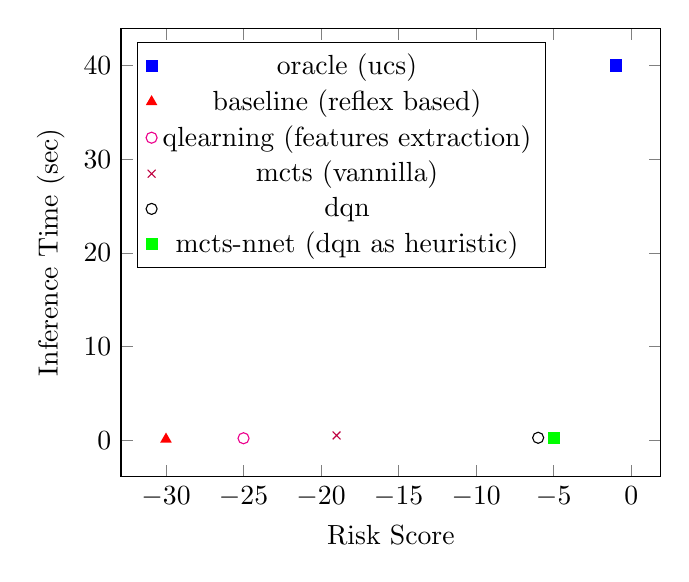
\begin{tikzpicture}
\begin{axis}[xlabel=Risk Score, ylabel=Inference Time (sec), legend pos=north west]
    \addplot[
        scatter,only marks,scatter src=explicit symbolic,
        scatter/classes={
            a={mark=square*,blue},
            b={mark=triangle*,red},
            c={mark=o,draw=magenta},
			d={mark=x,draw=purple},
			e={mark=o,draw=black,fill=black},
			f={mark=square*,green}
        }
    ]
    table[x=x,y=y,meta=label]{
        x    y    label
        -1    40.0  a
		-30   0.1   b
		-25   0.2   c
		-19   0.5   d
		-6    0.25  e
        -5    0.25  f
    };
    \legend{oracle (ucs),baseline (reflex based),qlearning (features extraction),mcts (vannilla),dqn,mcts-nnet (dqn as heuristic)}
\end{axis}
\end{tikzpicture}

\printbibliography

\end{document}
